\begin{frame}{R Markdown}

This is an R Markdown presentation. Markdown is a simple formatting
syntax for authoring HTML, PDF, and MS Word documents. For more details
on using R Markdown see \url{http://rmarkdown.rstudio.com}.

When you click the \textbf{Knit} button a document will be generated
that includes both content as well as the output of any embedded R code
chunks within the document.

\end{frame}

\begin{frame}{Slide with Bullets}

\begin{itemize}
\tightlist
\item
  Bullet 1
\item
  Bullet 2
\item
  Bullet 3
\end{itemize}

\end{frame}

\begin{frame}[fragile]{Slide with R Output}

\begin{Shaded}
\begin{Highlighting}[]
\KeywordTok{summary}\NormalTok{(cars)}
\end{Highlighting}
\end{Shaded}

\begin{verbatim}
##      speed           dist       
##  Min.   : 4.0   Min.   :  2.00  
##  1st Qu.:12.0   1st Qu.: 26.00  
##  Median :15.0   Median : 36.00  
##  Mean   :15.4   Mean   : 42.98  
##  3rd Qu.:19.0   3rd Qu.: 56.00  
##  Max.   :25.0   Max.   :120.00
\end{verbatim}

\end{frame}

\begin{frame}{Slide with Plot}

\includegraphics{Test2_files/figure-beamer/pressure-1.pdf}

\end{frame}

\section{jakldf}\label{jakldf}

\section{jakldf}\label{jakldf-1}

\section{jakldf}\label{jakldf-2}

\begin{frame}[fragile]{Parameter 2}

\begin{verbatim}
## [1] "c(1,1,1,1,1,1,1,1)"
\end{verbatim}

\end{frame}

\begin{frame}{Tabelle 1}

\begin{longtable}[c]{@{}ccc@{}}
\toprule
\begin{minipage}[b]{0.19\columnwidth}\centering\strut
Sepal.Length
\strut\end{minipage} &
\begin{minipage}[b]{0.18\columnwidth}\centering\strut
Sepal.Width
\strut\end{minipage} &
\begin{minipage}[b]{0.18\columnwidth}\centering\strut
Petal.Length
\strut\end{minipage}\tabularnewline
\midrule
\endhead
\begin{minipage}[t]{0.19\columnwidth}\centering\strut
5.1
\strut\end{minipage} &
\begin{minipage}[t]{0.18\columnwidth}\centering\strut
3.5
\strut\end{minipage} &
\begin{minipage}[t]{0.18\columnwidth}\centering\strut
1.4
\strut\end{minipage}\tabularnewline
\begin{minipage}[t]{0.19\columnwidth}\centering\strut
4.9
\strut\end{minipage} &
\begin{minipage}[t]{0.18\columnwidth}\centering\strut
3
\strut\end{minipage} &
\begin{minipage}[t]{0.18\columnwidth}\centering\strut
1.4
\strut\end{minipage}\tabularnewline
\begin{minipage}[t]{0.19\columnwidth}\centering\strut
4.7
\strut\end{minipage} &
\begin{minipage}[t]{0.18\columnwidth}\centering\strut
3.2
\strut\end{minipage} &
\begin{minipage}[t]{0.18\columnwidth}\centering\strut
1.3
\strut\end{minipage}\tabularnewline
\begin{minipage}[t]{0.19\columnwidth}\centering\strut
4.6
\strut\end{minipage} &
\begin{minipage}[t]{0.18\columnwidth}\centering\strut
3.1
\strut\end{minipage} &
\begin{minipage}[t]{0.18\columnwidth}\centering\strut
1.5
\strut\end{minipage}\tabularnewline
\begin{minipage}[t]{0.19\columnwidth}\centering\strut
5
\strut\end{minipage} &
\begin{minipage}[t]{0.18\columnwidth}\centering\strut
3.6
\strut\end{minipage} &
\begin{minipage}[t]{0.18\columnwidth}\centering\strut
1.4
\strut\end{minipage}\tabularnewline
\begin{minipage}[t]{0.19\columnwidth}\centering\strut
5.4
\strut\end{minipage} &
\begin{minipage}[t]{0.18\columnwidth}\centering\strut
3.9
\strut\end{minipage} &
\begin{minipage}[t]{0.18\columnwidth}\centering\strut
1.7
\strut\end{minipage}\tabularnewline
\bottomrule
\end{longtable}

\end{frame}

\begin{frame}{Tabelle 2}

\begin{longtable}[c]{@{}rrr@{}}
\toprule
Sepal.Length & Sepal.Width & Petal.Length\tabularnewline
\midrule
\endhead
5.1 & 3.5 & 1.4\tabularnewline
4.9 & 3.0 & 1.4\tabularnewline
4.7 & 3.2 & 1.3\tabularnewline
4.6 & 3.1 & 1.5\tabularnewline
5.0 & 3.6 & 1.4\tabularnewline
5.4 & 3.9 & 1.7\tabularnewline
\bottomrule
\end{longtable}

\end{frame}

\begin{frame}{Tikz}

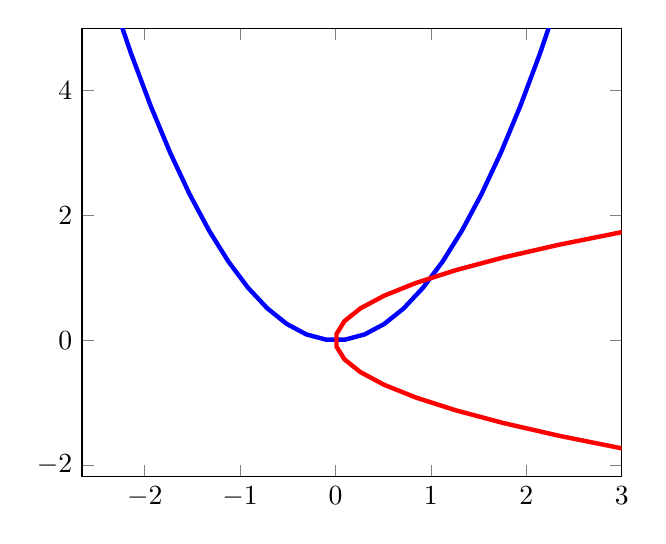
\begin{tikzpicture}
\begin{axis}[xmax=3,ymax=5, samples=50]
  \addplot[blue, ultra thick] (x,x*x);
  \addplot[red,  ultra thick] (x*x,x);
\end{axis}
\end{tikzpicture}

\end{frame}

\begin{frame}{Tikz 2}

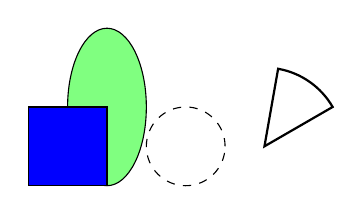
\begin{tikzpicture}
\draw[style=dashed] (2,.5) circle (0.5);
\draw[fill=green!50] (1,1)
ellipse (.5 and 1);
\draw[fill=blue] (0,0) rectangle (1,1);
\draw[style=thick]
(3,.5) -- +(30:1) arc(30:80:1) -- cycle;
\end{tikzpicture}

\end{frame}

\begin{frame}{Tikz 3}

\usetikzlibrary{backgrounds} \vspace*{-2.3cm}\hspace{8cm}\%

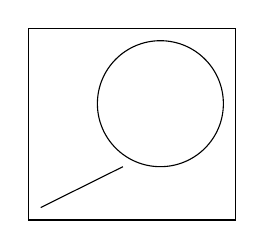
\begin{tikzpicture}[ scale=.8, show background rectangle]
\draw (2,2) circle (1);
\draw (1 mm, 10 pt) -- (4 em, 1);
\end{tikzpicture}

\end{frame}

\begin{frame}{Tikz 4}

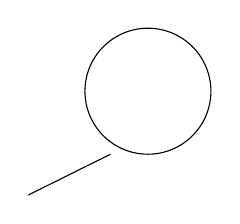
\begin{tikzpicture}[ scale=.8]
\draw (2,2) circle (1);
\draw (1 mm, 10 pt) -- (4 em, 1);
\end{tikzpicture}

\end{frame}

\begin{frame}{Tikz 5}

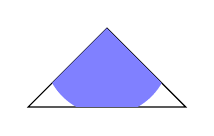
\begin{tikzpicture}
\path[clip, draw] (1,1)--(2,2)--(3,1)--cycle;
\path[fill=blue!50] (2, 1.7) circle (.8);
\end{tikzpicture}

\end{frame}

\begin{frame}{Tikz 6}

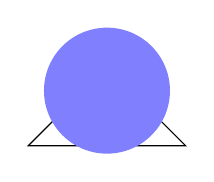
\begin{tikzpicture}
\path[draw] (1,1)--(2,2)--(3,1)--cycle;
\path[fill=blue!50] (2, 1.7) circle (.8);
\end{tikzpicture}

\end{frame}

\begin{frame}{Tikz 7}

\begin{tikzpicture}
\draw (0, 0) rectangle (7, 5);
\draw (3, 1) rectangle (1, 3);
\draw (3, 3) rectangle (1, 3);
\end{tikzpicture}

\end{frame}
